%
% Complete documentation on the extended LaTeX markup used for Insight
% documentation is available in ``Documenting Insight'', which is part
% of the standard documentation for Insight.  It may be found online
% at:
%
%     http://www.itk.org/

\documentclass{InsightArticle}

\usepackage[dvips]{graphicx}
%\usepackage{listing}						
\usepackage{listings}	
\usepackage{wrapfig}
\usepackage{amssymb,amsmath}
\usepackage{multirow,booktabs,array}
\usepackage{listings}
\usepackage{color}
				
%%%%%%%%%%%%%%%%%%%%%%%%%%%%%%%%%%%%%%%%%%%%%%%%%%%%%%%%%%%%%%%%%%
%
%  hyperref should be the last package to be loaded.
%
%%%%%%%%%%%%%%%%%%%%%%%%%%%%%%%%%%%%%%%%%%%%%%%%%%%%%%%%%%%%%%%%%%
\usepackage[
bookmarks,
bookmarksopen,
backref,
colorlinks,linkcolor={blue},citecolor={blue},urlcolor={blue},
]{hyperref}




\graphicspath{{./Figures/}}
\newcommand{\fv}{\mbox{\boldmath $f$}}
\newcommand{\Iv}{\mbox{\boldmath $I$}}
\newcommand{\xv}{\mbox{\boldmath $x$}}
\newcommand{\velocity}{\mbox{\boldmath $v$}}
\newcommand{\velocityinv}{\mbox{\boldmath $v$}^{-1}}
\newcommand{\Velocityinv}{\mbox{\boldmath $V$}^{-1}}
\newcommand{\Velocity}{\mbox{\boldmath $V$}}
\newcommand{\welocity}{\mbox{\boldmath $w$}}
\newcommand{\spatialimagegradient}{\mbox{\boldmath $I$}\mbox{$_{x}$}}
\newcommand{\perpspatialimagegradient}{\mbox{\boldmath $I$}\mbox{$^{\perp}_{x}$}}
\newcommand{\temporalimagederivative}{\mbox{$I_t$}}
\newcommand{\finitestrain}{\mbox{\boldmath $\varepsilon^{\ast}$}}
\newcommand{\smallstrain}{\mbox{\boldmath $\varepsilon$}}
\newcommand{\dispgradient}{{\bf \nabla \displace}}
\newcommand{\displace}{{\bf u}} 
\newcommand{\Id}{\text{\bf Id}}
\newcommand{\ode}{{\em O.D.E.}}
\newcommand{\odes}{{\em O.D.E.}s}
\newcommand{\G}{\mathcal{G}}
\newcommand{\J}{\mathcal{J}}
\newcommand{\phiinv}{\phi^{-1}}
\newcommand{\psiinv}{\psi^{-1}}
\newcommand{\dM}{DM}
\newcommand{\DM}{Diffeomorphometry}
\newcommand{\diff}{diffeomorphism}
\newcommand{\Diff}{Diffeomorphism}
\newcommand{\orbit}{\mathcal{O}}
\newcommand{\avg}{\mathcal{A}}
\newcommand{\avgn}{\mathcal{A}_n}
\newcommand{\avgna}{\mathcal{A}^a_{n}}
\newcommand{\nset}{\{ J_i \}_n}
\newcommand{\bari}{\bar{I}}
\newcommand{\bart}{\bar{t}}
\newcommand{\jac}{\mathcal{J}}
\newcommand{\pert}{\mbox{\boldmath $w$}}
\newcommand{\barpert}{\bar{\mbox{\boldmath $w$}}}
\newcommand{\half}{0.5}

\newcommand{\X}{{\bf X}}
\newcommand{\x}{{\bf x}}
\newcommand{\Z}{{\bf Z}}
\newcommand{\z}{{\bf z}}
\newcommand{\p}{{\bf p}}
\newcommand{\Y}{{\bf Y}}
\newcommand{\y}{{\bf y}}
\newcommand{\disp}{{\bf u}}
\newcommand{\ytild}{\tilde{{\bf y}}}
\newcommand{\q}{{\bf q}}
\newcommand{\surf}{\mathcal{S}}
\newcommand{\phij}{\phi_{ij}}
\newcommand{\aphij}{\bar{\phi}_{j}}
\newcommand{\apsij}{\bar{\psi}_{j}}
\newcommand{\aphi}{\bar{\phi}}
\newcommand{\aphiinv}{\bar{\phi}^{-1}}

\newcommand{\domain}{\Omega}
\newcommand{\meanshape}{\bf \bar{x}}
\newcommand{\g}{\mbox{\boldmath $g$}}
\newcommand{\h}{\mbox{\boldmath $h$}}
\newcommand{\yv}{\mbox{\boldmath $y$}}

\newcommand{\group}{Diff}


\newcommand{\evol}{{E_{\text{Vol}}}}
\newcommand{\epair}{{E_{\text{Pair}}}}
\newcommand{\esec}{{E_{S}}}
\newcommand{\inv}{^{-1}}
\newcommand{\vinit}{ \velocity^0_{ij}(\x,\tau=0) }
\newcommand{\avinit}{ \bar{\velocity}^0_{j}(\x,t) }
\newcommand{\avinitz}{ \bar{\velocity}^0_{j}(\x,t_a) }
\newcommand{\gz}{\nabla_{\z}}


 
\definecolor{dkgreen}{rgb}{0,0.6,0}
\definecolor{gray}{rgb}{0.5,0.5,0.5}
\definecolor{mauve}{rgb}{0.58,0,0.82}

\lstset{ %
  language=bash,                % the language of the code
  basicstyle=\footnotesize,           % the size of the fonts that are used for the code
  numbers=left,                   % where to put the line-numbers
  numberstyle=\tiny\color{gray},  % the style that is used for the line-numbers
  stepnumber=2,                   % the step between two line-numbers. If it's 1, each line 
                                  % will be numbered
  numbersep=5pt,                  % how far the line-numbers are from the code
  backgroundcolor=\color{white},      % choose the background color. You must add \usepackage{color}
  showspaces=false,               % show spaces adding particular underscores
  showstringspaces=false,         % underline spaces within strings
  showtabs=false,                 % show tabs within strings adding particular underscores
  frame=single,                   % adds a frame around the code
  rulecolor=\color{black},        % if not set, the frame-color may be changed on line-breaks within not-black text (e.g. commens (green here))
  tabsize=2,                      % sets default tabsize to 2 spaces
  captionpos=b,                   % sets the caption-position to bottom
  breaklines=true,                % sets automatic line breaking
  breakatwhitespace=true,        % sets if automatic breaks should only happen at whitespace
  prebreak=\textbackslash, breakindent=7pt,
  title=\lstname,                   % show the filename of files included with \lstinputlisting;
                                  % also try caption instead of title
  keywordstyle=\color{blue},          % keyword style
  commentstyle=\color{dkgreen},       % comment style
  stringstyle=\color{mauve},         % string literal style
  escapeinside={\%*}{*)},            % if you want to add a comment within your code
  morekeywords={*,...}               % if you want to add more keywords to the set
}

\lstdefinestyle{bash}{language=bash} 
\lstdefinestyle{perl}{language=perl} 

%  This is a template for Papers to the Insight Journal. 
%  It is comparable to a technical report format.

% The title should be descriptive enough for people to be able to find
% the relevant document. 
\title{The PipeDream Neuroimaging Pipeline for Cross-Sectional and Longitudinal Studies of Cortex and Connectivity}

% 
% NOTE: This is the last number of the "handle" URL that 
% The Insight Journal assigns to your paper as part of the
% submission process. Please replace the number "1338" with
% the actual handle number that you get assigned.
%
%\newcommand{\IJhandlerIDnumber}{}

% Increment the release number whenever significant changes are made.
% The author and/or editor can define 'significant' however they like.
\release{0.1}

% At minimum, give your name and an email address.  You can include a
% snail-mail address if you like.
\author{P.Cook, B. Avants, N. Tustison, J. Duda, J. Gee}
\authoraddress{Penn Image Computing And Science Laboratory\\
University of Pennsylvania}

\begin{document}

%
% Add hyperlink to the web location and license of the paper.
% The argument of this command is the handler identifier given
% by the Insight Journal to this paper.
% 
%\IJhandlefooter{\IJhandlerIDnumber}


\ifpdf
\else
   %
   % Commands for including Graphics when using latex
   % 
   \DeclareGraphicsExtensions{.eps,.jpg,.gif,.tiff,.bmp,.png}
   \DeclareGraphicsRule{.jpg}{eps}{.jpg.bb}{`convert #1 eps:-}
   \DeclareGraphicsRule{.gif}{eps}{.gif.bb}{`convert #1 eps:-}
   \DeclareGraphicsRule{.tiff}{eps}{.tiff.bb}{`convert #1 eps:-}
   \DeclareGraphicsRule{.bmp}{eps}{.bmp.bb}{`convert #1 eps:-}
   \DeclareGraphicsRule{.png}{eps}{.png.bb}{`convert #1 eps:-}
\fi


\maketitle


\ifhtml
\chapter*{Front Matter\label{front}}
\fi



% The abstract should be a paragraph or two long, and describe the
% scope of the document.
\begin{abstract}
\noindent PipeDream uses open-source software to help neuroimaging researchers perform advanced processing with state-of-the-art techniques.  PipeDream performs data reconstruction, data organization, advanced brain extraction, bias correction, three tissue classification and cortical thickness estimation.  Diffusion tensor processing, unbiased longitudinal analysis and cortical parcellation are available as advanced options.  PipeDream relies on prior knowledge encoded in an optimal template.  PipeDream also helps one review the processing and perform quality assurance.  The tool documents our current ``best practice'', implementable with free software, for MRI-based studies of the brain.
\end{abstract}

%\IJhandlenote{\IJhandlerIDnumber}

\tableofcontents
\newpage
\section*{Introduction}

For the latest updates to the code and this document, please see the PipeDream online repository at \url{https://github.com/cookpa/pipedream}. 

This document covers the installation of PipeDream and related software, and the use of the PipeDream tools to process an example data set.


\section{Documentation and getting help}

This document is designed to help you get up and running using PipeDream. You can get additional help on the command line by running any command without any arguments. If you need further assistance or have any feedback, contact us at \url{mailto:cookpa@mail.med.upenn.edu}.

\section{Installation}

PipeDream assumes the basic unix tools that exist on GNU / Linux. On most Linux installations, everything you need to carry out installation will be available by default. 

The instructions below explain how to obtain and build the software we use in PipeDream. Some of these tools are not affiliated in any way with PipeDream or the PICSL lab. They come with their own licensing agreements, which can be found at the web pages for each tool given below. Since PipeDream is an open-source pipeline, we've chosen to integrate only tools that are freely available (and preferably open source) for academic use.

\subsection{Prerequisites on Mac OS X}

PipeDream can run on a Mac OS X system, however you may need to install some extra software. Install Xcode, which provides the necessary compilers, git, and other useful tools. Next, we recommend the Homebrew package manager \url{http://mxcl.github.com/homebrew/}. 

Mac OS X is based on BSD Unix, so there may be some differences in the implementation of unix tools. As of 10.7 (Lion), there are no known incompatibilities with PipeDream. However, you may optionally install the GNU Core Utils, which you can do with Homebrew:
\begin{lstlisting}[style=bash]
  brew install coreutils
\end{lstlisting}

This will install the GNU tools, however they will be prefixed with a g, so ``ls" will be called ``gls" and so on. You can create symlinks in \code{/usr/local/bin} to get around this, such that ``ls" etc point to the GNU tools.    


\subsection{CMake}

CMake is required for compiling ITK, ANTS, and GDCM, among other things. It can be downloaded from its website \url{http://cmake.org/}. Hombrew users can install it by typing \code{brew install cmake}.

CMake is a very powerful tool, and will do lots of configuration behind the scenes to enable code compilation on your machine. We will just need to know how to use the \code{ccmake} program. The options presented to you in CMake may differ slightly across platforms. For example, on Mac you will be asked which version of OS X to target, but overall the build process is very similar. This is the beauty of CMake, under the hood building on different systems is very different, but with CMake almost all of the necessary work is done for you.


\subsection{ITK}

The first thing you'll need to compile is ITK. At the time of writing, both ITK and ANTS are in a development phase, so you'll want to use the latest stable ITK. Clone the repository with git and checkout the nightly-master branch.
\begin{lstlisting}[style=bash]
  mkdir ~/src
  cd ~/src
  git clone http://itk.org/ITK.git
  git checkout -b my_nightly_master origin/nightly-master
\end{lstlisting}
The above only needs to be done once, to update the source later you can update by pulling the remote nightly-master:
\begin{lstlisting}[style=bash]
  git pull origin nightly-master
\end{lstlisting}

More information about git can be found in the free online git book \url{http://git-scm.com/book}.

Once the source code is checked out, we will proceed to build. We always build outside the source tree.
\begin{lstlisting}[style=bash]
  mkdir -p ~/bin/itk
  cd ~/bin/itk
  ccmake ~/src/ITK
\end{lstlisting}
This will bring up the \code{ccmake} interface. Initially, you will see the message \code{EMPTY CACHE}, meaning CMake hasn't done any configuration yet. Hit C to do an initial configuration. CMake will choose as many settings as it can automatically, and present others to you for review. Navigate to the options and hit enter to toggle boolean options or to enter text where needed.  Turn off building examples and testing to save compilation time. Make sure the \code{CMAKE\_BUILD\_TYPE} says ``Release" - this is important for ANTS too, since debug code is substantially slower. Also make sure that \code{ITK\_BUILD\_ALL\_MODULES} is on. Hit C again to reconfigure. You should now have a CMake screen that looks like figure \ref{fig:itkCCMake}. Hit G to generate the make files and exit. 

Back at the terminal, you can now start compilation with \code{make}.

\begin{figure}
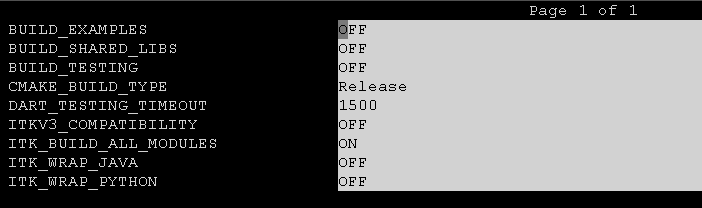
\includegraphics[width=0.8\textwidth]{figures/itk_ccmake.png} 
\itkcaption[ITK CCMake screen]{ITK configured in \code{ccmake}.}
\label{fig:itkCCMake}
\end{figure}


\subsection{ANTS}

ANTS will be checked out and built in a similar way to ITK, except that we use Subversion instead of git (in the future, ANTS will move to git).
\begin{lstlisting}[style=bash]
cd ~/src
svn checkout https://advants.svn.sourceforge.net/svnroot/advants/trunk ants
mkdir ~/bin/ants
cd ~/bin/ants
ccmake ~/src/ants/Examples
\end{lstlisting}
As before, set \code{BUILD\_TESTING} off and ensure that the build type is set to ``Release". Reconfigure until everything is set, then generate the makefiles and make.

After building ANTS, it's a good idea to record the version information of ANTS and ITK. This will help the developers reproduce any bugs or performance issues you encounter. Record the source code version information with \code{git} and \code{svn}.
\begin{lstlisting}[style=bash]
cd ~/src/ITK
git show > ~/bin/ants/version_info.txt
svn info ~/src/ants >> ~/bin/ants/version_info.txt 
\end{lstlisting}


\subsection{GDCM}

GDCM is available through Sourceforge, which means you can get it using Git or by downloading a tarball from its website \url{http://sourceforge.net/projects/gdcm/}. It builds with CMake. Building should be straightforward following the procedure above. Set \code{GDCM\_BUILD\_APPLICATIONS} on, PipeDream needs these applications to parse DICOM headers.

\subsection{MRIcron}

MRIcron is distributed in binary form from its web page \url{http://www.nitrc.org/projects/mricron}. The package contains several tools, including the \code{mricron} image viewer and the \url{npm} statistical tool. In PipeDream we use the \code{dcm2nii} program that converts DICOM series to NIFTI images.

\subsection{Camino}

Camino is a diffusion MRI toolkit. It can be downloaded from \url{http://camino.org.uk}. It builds directly from the package, assuming you have Oracle Java installed.
\begin{lstlisting}[style=bash]
cd ~/bin/
tar -xzvf /path/to/camino.tgz
cd camino
make
\end{lstlisting}


\subsection{Other tools}

These tools are not required by PipeDream but may be useful to many users.

\subsubsection{ITK-SNAP}

ITK-SNAP is useful for image viewing and segmentation, and is avaliable from \url{http://www.itksnap.org}.

\subsubsection{convert3d}

The \code{c3d} command wraps many of the image processing filters of ITK in a command-line tool. It can handle complex operations in memory using an operations stack. See \url{http://www.itksnap.org/pmwiki/pmwiki.php?n=Convert3D.Convert3D}.


\subsection{PipeDream}

\begin{lstlisting}[style=bash]
  cd ~/bin
  git clone git://github.com/cookpa/pipedream.git
  cd pipedream
  git checkout -b mybranch origin/master
  cp config/pipedream_config_example.sh config/pipedream_config.sh
\end{lstlisting}

Edit the \code{config/pipedream\_config.sh} file. Most of the variables are paths to the other software mentioned above. You should also review the \code{qsub} command that will be used to submit jobs to the queue. 

Add the \code{pipedream/bin} directory to your PATH.
\begin{lstlisting}[style=bash]
 export PATH=/path/to/pipedream/bin:$PATH
\end{lstlisting}
You can add this line to your \code{.bash\_profile} to give you access to PipeDream at login.
 

\section{Running the pipelines}

The pipedream neuroimaging pipeline has five stages: 
\begin{enumerate}
\item Organize data
\item Pre-process individual modality images
\item Construct a template.  
\item Run the brain processing pipeline.  
\item Check results. 
\item Perform statistical analyses.  
\end{enumerate}

We cover each step in turn in the following sections. \footnote{This document is a work in progress. Please check for updates with each release.}

\section{Example data}

At various points in this document we make use of the example data in \code{pipedream/testing/data} directory.

% Git instructions on submodule here

The Kirby data comes from the F.M. Kirby Center Multi?Modal Reproducbility Study at the Kennedy Krieger Institute, and is distributed under the BIRN data license. More information, and access to the complete set of raw data are at \url{http://www.nitrc.org/projects/multimodal}. 



% OR - just organize and upload the data


\section{Data Organization and study design}

PipeDream is designed to work with DICOM data, and contains tools for properly organizing DICOM files and converting them to NIFTI-1 format. If you do not have access to DICOM data, you can replicate the data organization and pick up the pipeline at the NIFTI stage, see \ref{sec:dicom2nii}.

In all processing, images are identified by a unique subject identifier and a scan date. Subject identifiers are chosen by the user. They should be alphanumeric and not include special characters that may cause problems for scripts. Alphanumeric includes all letters and numbers, plus the underscore character \_. Other characters have special meaning in various software packages and may cause problems. 

The choice of subject identifiers should be consistent for imaging and non-imaging data that will be part of your study. 


\subsection{DICOM data organization}

PipeDream organizes DICOM data from a given subject by date and series number. It does not sort subjects by subject identifier, because the correct choice of identifier is often not present the header. The user needs to choose the subject identifier at run time. The rest of the organization can be done by \code{dicom2series}.

In the absence of public data in DICOM format, we will use a hypothetical example data set. We have a base directory \code{\$RAW\_DICOM\_DIR} that contains subjects numbered 001 through 100. Within \code{\$RAW\_DICOM\_DIR/001}, the DICOM data for subject 001 is stored in some unknown format, perhaps copied from a CD written at the scanner. We can process all the data with the following script.
\begin{lstlisting}[style=bash]
 for subj in `seq -w 1 100`; do
   find -L ${RAW_DICOM_DIR}/$subj -type f -print0 | xargs -0 dicom2series ~/subjectsDICOM/$subj 1 0 
 done
\end{lstlisting}
Here we use the \code{find} utility to list all files within each subject's data directory. The use of \code{-print0} and \code{xargs} make the command robust to large numbers of files, and spaces in the file or directory names. Non-DICOM files will be skipped automatically. 

DICOM index files can sometimes confuse \code{dicom2series}. These are usually files called \code{DICOMDIR}. If they are present you can remove them from the above command by adding \code{-not -name DICOMDIR} to the \code{find} command above.

The output data will be organized hierarchically by subject, acquisition time, and then by series. The subject identifier is completely under the user's control and is specified on the command line. The acquisition time is determined from the data and is written in the format YYYY\_MM\_DD\_HHMM where the first three items are the study date, and the final ``HHMM" is hour and minute of the study time. The series are named by series number, protocol name, and series description, in the format NUMBER\_PROTOCOL\_DESCRIPTION. The output DESCRIPTION is the concatenation of the protocol name and series description in the data, minus any duplication. Thus if your protocol name is ``DTI30DIR" and your series description is ``DTI30DIR\_ADC" the output description will be ``DTI30DIR\_ADC" not ``DTI30DIR\_DTI30DIR\_ADC".


\section{DICOM to NIFTI conversion} \label{sec:dicom2nii}

We recommend keeping the NIFTI data in a separate directory structure. The first thing we do is define a list of protocols that should be converted. That is, the name of protocols as they appear in the \code{subjectsDICOM} directory, minus the series numbers. These should be written to a text file, let's say \code{all\_protocols.txt}, one per line, for example
\begin{lstlisting}[style=bash]
t1_mpr_AX_MPRAGE
t2_tse_obl_448_2mm
DTI_30dir_noDiCo_vox2_1000
DTI_34dir
\end{lstlisting}

Next, list the subjects that need processing. Usually this will be every subject listed in \code{subjectsDICOM/}
\begin{lstlisting}[style=bash]
  ls subjectsDICOM > subjects.txt  
\end{lstlisting}

Now we're ready to run
\begin{lstlisting}[style=bash]
 dicom2nii sge subjects.txt  all_protocols.txt subjectsDICOM subjects
\end{lstlisting}

The output is organized in \code{subjects/subjectID/time/rawNii}. For example, \code{subjects/104391/2007\_07\_10\_1024/rawNii}, which contains:
\begin{lstlisting}[style=bash]
104391_2007_07_10_1024_0006_t1_mpr_AX_MPRAGE.nii.gz
104391_2007_07_10_1024_0011_DTI_30dir_noDiCo_vox2_1000.bval
104391_2007_07_10_1024_0011_DTI_30dir_noDiCo_vox2_1000.bvec
104391_2007_07_10_1024_0011_DTI_30dir_noDiCo_vox2_1000.nii.gz
104391_2007_07_10_1024_0013_DTI_30dir_noDiCo_vox2_1000.bval
104391_2007_07_10_1024_0013_DTI_30dir_noDiCo_vox2_1000.bvec
104391_2007_07_10_1024_0013_DTI_30dir_noDiCo_vox2_1000.nii.gz
104391_2007_07_10_1024_0015_DTI_30dir_noDiCo_vox2_1000.bval
104391_2007_07_10_1024_0015_DTI_30dir_noDiCo_vox2_1000.bvec
104391_2007_07_10_1024_0015_DTI_30dir_noDiCo_vox2_1000.nii.gz
\end{lstlisting}
The protocol ``t1\_mpr\_AX\_MPRAGE" is a T1 protocol, so the output is a 3D NIFTI image. The protocol ``DTI\_30dir\_noDiCo\_vox2\_1000" is a diffusion protocol, so the output is 4D, and there are two additional files that describe the diffusion gradient vectors.

If your raw data is already in NIFTI format, you can begin processing with PipeDream at this point by copying your data into the structure above. The series numbers can be assigned arbitrarily. The acquisition date can be specified in a format of your choice, we recommend ``YYYY\_MM\_DD", because then the text sorts in the correct temporal order. If you don't have DICOM data you probably won't know study time, but that's only a problem if you have multiple same-day imaging sessions. If that's the case, then you should add ``\_0001", ``\_0002", etc in place of the study time.

In the following sections, we discuss the various programs that do modality-specific pre-processing for the different images that PipeDream supports.


\section{Modality specific preprocessing - scalar images}

Scalar images, for example a T1 MRI, do not require any specialized pre-processing, however it is often convenient to rename them into a common format.


\section{Modality specific preprocessing - diffusion images}

The basic preprocessing steps for diffusion images are
\begin{enumerate}
\item Affine normalization of DWI images to the first b=0 image, for motion and distortion correction. 
\item Registration of the average DWI image to a template, to define the brain mask.
\item Reconstruction of the diffusion tensor by weighted linear regression.
\item Computation of FA, MD, RGB images.
\end{enumerate}
A full list of the output generated by nii2dt is given in table \ref{t/l:nii2dtout}.

\subsection{Kirby data example}

\begin{table}[htdp]
\caption{default}
\begin{center}
\begin{tabular}{|c|c|}
\hline
\textbf{Output} & \textbf{Description} \\ \hline
allscans.scheme & The scheme file for the complete acquisition, including repeats if any. \\ \hline
averagedwi.nii.gz & The average of all images with $b > 0$. \\ \hline
brainmask.nii.gz & The brain / background binary mask, computed by registering the average DWI to a template. \\ \hline
dt.nii.gz         & The diffusion tensors in NIfTI format. \\ \hline
dwi               & Directory containing corrected raw DWI images \\ \hline
exitcode.nii.gz   & Contains brain / background mask and flags for bad data. \\ \hline
fa.nii.gz            & Fractional anisotropy \\ \hline
lns0.nii.gz       & Reconstructed estimate of the log of the b=0 signal. \\ \hline
md.nii.gz          & Mean diffusivity. Units are dependent on the input b-values, which are usually $\textrm{s} / \textrm{mm}^2$.
rgb.nii.gz           & Color coded 
sigmaSq.nii.gz    & Estimate of the noise variance in each voxel \\ \hline
\end{tabular}
\end{center}
\label{tbl:nii2dtout}
\caption{Output of nii2dt}
\end{table}%

% Other pre-processing goes here


\section{Automating preprocessing}




\section{Construct a Template}
Pipedream requires that you have a template---preferably constructed
from a dataset similar to your current study---with a number of
companion images that contain anatomical labels.  The minimum set of
priors include: a brain or cerebrum mask, a cerebrospinal fluid
probability map, a gray matter probability map and white matter
probability map.

If you do not have a template already available---or would like a local/optimal 
template---then you can build one from your data by following these steps:
\begin{enumerate}
\item Create a template directory where you can write a bunch of data.
\item Link your anatomical (T1-MRI) images into the directory, using ``ln -s'' in unix/linux/osx.
\item Call the ANTS command AverageImages to get an initial template
  or copy one of your subjects to a file called DIFFtemplate.nii.gz
  .... Make sure you don't copy a file called image.nii to a nii.gz
  file-type.  Either way, you will get an unbiased template out of this process.  
\item Call the ANTS script :   sh buildtemplateparallel.sh in this directory.  
  An example call is here: 
\begin{verbatim}
  sh buildtemplateparallel.sh -d 3 -o DIFF -c 2 -j 2 -z DIFFtemplate.nii.gz  *T1.nii.gz 
\end{verbatim}
  In this example, we assume you have images of the type   Sub001T1.nii.gz .
  Note that the buildtemplateparallel script is a complex algorithm in itself and takes time.  
  If you can get a pre-built template, then that would be preferable. 
\item  Extract the brain from the output template (using, for instance, www.itksnap.org) and segment it into three tissue classes.  
  The ANTS Atropos tool will allow you to do this.  However, this should be done well in that 
  it will impact your study outcome.   Keep the four label/probability images you generated for use as priors in your study. 
  See the file pipedreamsegment3classnowarp.sh in pipedream to see how one might achieve a good segmentation of an image 
  in a stand-alone module.  
\end{enumerate}
It takes some effort to produce a good template.  So, check with developers to see 
if one is available for your type of data.

\begin{figure}
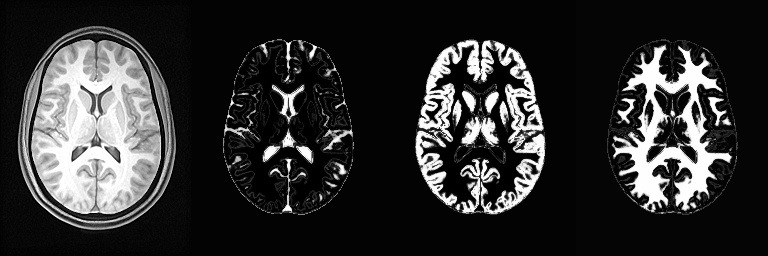
\includegraphics[width=0.9\textwidth]{figures/templatefig.jpg} 
\itkcaption[Template Prior]{An example template.}
\vspace{-0.1in}
\label{fig:template}
\end{figure}

\section{Run a Cross-Sectional Study}
To run a pipedream study, your data needs to be organized as above and you need a template 
with all the necessary prior information available.  When all is ready, you will call:
\begin{verbatim}
    sh $PIPEDREAMDIR/pipedreamMapT1.sh pipedreamMapT1paramsUser.sh 
\end{verbatim}
where you likely have copied the ``base'' pipedreamMapT1paramsUser.sh
to your local directory and edited it for your data.  The output
directory structure and naming will mirror your input structure.  You
will get cortical thickness images, brain extraction, probability
maps, estimates of brain volume and---if enabled---a cortical
parcellation.

The key to the study is the file pipedreamMapT1paramsUser.sh.  
Within that file is a series of directory and then file variables that you need to define.  
We've tried to ``check'' your definitions for you and provide a warning that will help you 
find a mistake but this may not always work.  So, take care when making these definitions.

An important part of this step is how you distribute these processes.
We provide hooks for voxbo and for the SGE qsub.  There is also a
PIPEDREAMISTEST variable in the user configuration file that will set
``fast'' parameters to allow you to check your configuration before
running the full dataset.  Set variable GOTOVBQ=1, GOTOSGEQ=0 (for
voxbo) GOTOVBQ=0, GOTOSGEQ=1 (for sge) in pipedreamMapT1paramsUser.sh.  
If both are zero, you will run in serial mode. 

\section{Check Results}

Pipedream output is organized by subject and time point in a similar way to the input data, except that structural and DTI data are placed in the same directory. Within each time point output directory, there are the following files, prefixed with the subject ID and time point ID.

Images suffixed with ``norm.nii.gz" are normalized to standard space. If a mapping from the local template to standard space is provided, then all ``norm.nii.gz" are in standard space. Otherwise they are in the local template space. The images relating to DT processing are only produced if you have DT data for the subject and time point.

\begin{table}[htdp]
\caption{default}
\begin{center}
\begin{tabular}{| p{5cm} | p{10cm} |}
\hline
\textbf{Output} & \textbf{Description} \\ \hline
Affine.txt, InverseWarp.nii.gz, Warp.nii.gz & Warps from subject T1 to local template space. \\ \hline
brain.nii.gz & The brain-extracted and bias-corrected T1 image in subject space. \\ \hline
brainmask.nii.gz & The brain mask of the T1 image, used to compute brain.nii.gz. \\ \hline
brain\_prob\_[0,1,2].nii.gz & Segmentation probabilities of CSF (0), gray matter (1) and white matter in the T1 image. \\ \hline
deformed.nii.gz & Input head image deformed to the local template space. Useful for evaluating brain extraction and registration. \\ \hline
distcorr[Affine.txt, Warp.nii.gz, InverseWarp.nii.gz] & Distortion correction between T1 and DT space.\\ \hline
DTdeformed.nii.gz & DT image warped to the local template space \\ \hline
fa.nii.gz & Fractional anisotropy from DTI, in the subject space. \\ \hline
fadeformed.nii.gz & FA deformed into the local template space. \\ \hline
gmpnorm.nii.gz         & Normalized gray matter probability (brain\_prob\_1.nii.gz). \\ \hline
grid.nii.gz & Deformation grid showing the warp of the T1 image to template space. Used for evaluating registration. \\ \hline
head.nii.gz & Input T1 image. \\ \hline
kappa.nii.gz               & White matter curvature. \\ \hline
kappanorm.nii.gz   & kappa transformed to standard space. \\ \hline
logjacobian.nii.gz   & Log determinant of the Jacobian, in the local template space. \\ \hline
seg.nii.gz      & Three tissue segmentation of the T1 brain image.\\ \hline
thickness.nii.gz & Cortical thickness in the subject space. \\ \hline
thicknorm.nii.gz & Thickness warped to standard space. \\ \hline
\end{tabular}
\end{center}
\label{pipedreamMapT1out}
\caption{Output of pipedreamMapT1}
\end{table}%

If you have defined label images in the template space, there will be additional output containing the labels and probabilities in the subject space.

It's critical to evaluate the output data visually before doing statistics. The normalized images can be evaluated by extracting the same slice from all subjects, using ANTS:
\begin{verbatim}
    $ANTSPATH/StackSlices vol.nii.gz -1 -1 80  PipeDreamOutDir/*/*/*_thickness.nii.gz
\end{verbatim}
This will extract the 80th z-slice of every image and put it into a volume (vol.nii.gz) 
that you can scroll through.  You can call this on any image type.  If some specific dataset, e.g. subject00X, does not work, you 
may want to manually set the variable PIPEDREAMSUBJECTSLIST=subject00X and run a test 
on that subject alone, without sending to distributed computing, to see what is going on.  As above, if you 
set PIPEDREAMISTEST=1 you can get a fast test result for this subject.  

\section{Compute Statistics} 
If everything is good, you are ready to estimate group statistics.  We
prefer a {\bf R} statistical interface and can provide a script for
you.  However, you may run your favorite statistical package on the
output of pipedream.

\begin{comment}
\section{The PipeDream Preprocessing Pipeline} 
\subsection{Data Organization}
\subsection{T1 Pipeline} 
\subsection{DTI Pipeline}
\subsection{Quality Assurance}

\section{The PipeDream Cross-sectional Pipeline}

\subsection{The Importance of the Template}
\subsection{Customization}
\subsection{Required Software}

\section{The PipeDream Longitudinal Pipeline}

\section{A Working Example}
\subsection{The Template}
\subsection{The Data}
\subsection{The Results}
\subsection{The Longitudinal Results}
\end{comment}

\section{Annotated Bibliography}
The original statement of the symmetric normalization and template
construction methodology was given in \cite{Avants2004}.  A follow up
study that used landmark guidance to compare the chimpanzee cortex to
the human cortex was published here \cite{Avants2006} -- this study
used {\em in vivo} MRI and template-based normalization to confirm
volumetric numbers derived from an early 20th century post-mortem
study comparing one human and one chimp.  This conference article has
some additional detail and alternative updates to the methodology, in
particular application to shape-based interpolation
\cite{Avants2005b}.  Network based studies were performed here
\cite{duda08miccai,duda08cvpr}.  The main SyN paper is here
\cite{Avants2008}.  Applications to neurodegeneration are here
\cite{Avants2005,Avants2008a,Grossman2008,Avants2009,Das2009,Yushkevich2009,Massimo2009}.
Hippocampus focused work is here \cite{Pluta2009,Yushkevich2009}.  The
main evaluation papers include \cite{Avants2008} and \cite{Klein2009}
for the cortex and deep brain structures whereas \cite{Pluta2009}
evaluates the use of automated and semi-automated normalization for
high-throughput hippocampus morphometry.  An additional evaluation
paper is being developed.  


%%%%%%%%%%%%%%%%%%%%%%%%%%%%%%%%%%%%%%%%%
%
%  Insert the bibliography using BibTeX
%
%%%%%%%%%%%%%%%%%%%%%%%%%%%%%%%%%%%%%%%%%

\bibliographystyle{plain}
\bibliography{references,ants}


\end{document}

